\documentclass[11pt]{article}

    \usepackage[breakable]{tcolorbox}
    \usepackage{parskip} % Stop auto-indenting (to mimic markdown behaviour)
    
    \usepackage{iftex}
    \ifPDFTeX
    	\usepackage[T1]{fontenc}
    	\usepackage{mathpazo}
    \else
    	\usepackage{fontspec}
    \fi

    % Basic figure setup, for now with no caption control since it's done
    % automatically by Pandoc (which extracts ![](path) syntax from Markdown).
    \usepackage{graphicx}
    % Maintain compatibility with old templates. Remove in nbconvert 6.0
    \let\Oldincludegraphics\includegraphics
    % Ensure that by default, figures have no caption (until we provide a
    % proper Figure object with a Caption API and a way to capture that
    % in the conversion process - todo).
    \usepackage{caption}
    \DeclareCaptionFormat{nocaption}{}
    \captionsetup{format=nocaption,aboveskip=0pt,belowskip=0pt}

    \usepackage[Export]{adjustbox} % Used to constrain images to a maximum size
    \adjustboxset{max size={0.9\linewidth}{0.9\paperheight}}
    \usepackage{float}
    \floatplacement{figure}{H} % forces figures to be placed at the correct location
    \usepackage{xcolor} % Allow colors to be defined
    \usepackage{enumerate} % Needed for markdown enumerations to work
    \usepackage{geometry} % Used to adjust the document margins
    \usepackage{amsmath} % Equations
    \usepackage{amssymb} % Equations
    \usepackage{textcomp} % defines textquotesingle
    % Hack from http://tex.stackexchange.com/a/47451/13684:
    \AtBeginDocument{%
        \def\PYZsq{\textquotesingle}% Upright quotes in Pygmentized code
    }
    \usepackage{upquote} % Upright quotes for verbatim code
    \usepackage{eurosym} % defines \euro
    \usepackage[mathletters]{ucs} % Extended unicode (utf-8) support
    \usepackage{fancyvrb} % verbatim replacement that allows latex
    \usepackage{grffile} % extends the file name processing of package graphics 
                         % to support a larger range
    \makeatletter % fix for grffile with XeLaTeX
    \def\Gread@@xetex#1{%
      \IfFileExists{"\Gin@base".bb}%
      {\Gread@eps{\Gin@base.bb}}%
      {\Gread@@xetex@aux#1}%
    }
    \makeatother

    % The hyperref package gives us a pdf with properly built
    % internal navigation ('pdf bookmarks' for the table of contents,
    % internal cross-reference links, web links for URLs, etc.)
    \usepackage{hyperref}
    % The default LaTeX title has an obnoxious amount of whitespace. By default,
    % titling removes some of it. It also provides customization options.
    \usepackage{titling}
    \usepackage{longtable} % longtable support required by pandoc >1.10
    \usepackage{booktabs}  % table support for pandoc > 1.12.2
    \usepackage[inline]{enumitem} % IRkernel/repr support (it uses the enumerate* environment)
    \usepackage[normalem]{ulem} % ulem is needed to support strikethroughs (\sout)
                                % normalem makes italics be italics, not underlines
    \usepackage{mathrsfs}
    

    
    % Colors for the hyperref package
    \definecolor{urlcolor}{rgb}{0,.145,.698}
    \definecolor{linkcolor}{rgb}{.71,0.21,0.01}
    \definecolor{citecolor}{rgb}{.12,.54,.11}

    % ANSI colors
    \definecolor{ansi-black}{HTML}{3E424D}
    \definecolor{ansi-black-intense}{HTML}{282C36}
    \definecolor{ansi-red}{HTML}{E75C58}
    \definecolor{ansi-red-intense}{HTML}{B22B31}
    \definecolor{ansi-green}{HTML}{00A250}
    \definecolor{ansi-green-intense}{HTML}{007427}
    \definecolor{ansi-yellow}{HTML}{DDB62B}
    \definecolor{ansi-yellow-intense}{HTML}{B27D12}
    \definecolor{ansi-blue}{HTML}{208FFB}
    \definecolor{ansi-blue-intense}{HTML}{0065CA}
    \definecolor{ansi-magenta}{HTML}{D160C4}
    \definecolor{ansi-magenta-intense}{HTML}{A03196}
    \definecolor{ansi-cyan}{HTML}{60C6C8}
    \definecolor{ansi-cyan-intense}{HTML}{258F8F}
    \definecolor{ansi-white}{HTML}{C5C1B4}
    \definecolor{ansi-white-intense}{HTML}{A1A6B2}
    \definecolor{ansi-default-inverse-fg}{HTML}{FFFFFF}
    \definecolor{ansi-default-inverse-bg}{HTML}{000000}

    % commands and environments needed by pandoc snippets
    % extracted from the output of `pandoc -s`
    \providecommand{\tightlist}{%
      \setlength{\itemsep}{0pt}\setlength{\parskip}{0pt}}
    \DefineVerbatimEnvironment{Highlighting}{Verbatim}{commandchars=\\\{\}}
    % Add ',fontsize=\small' for more characters per line
    \newenvironment{Shaded}{}{}
    \newcommand{\KeywordTok}[1]{\textcolor[rgb]{0.00,0.44,0.13}{\textbf{{#1}}}}
    \newcommand{\DataTypeTok}[1]{\textcolor[rgb]{0.56,0.13,0.00}{{#1}}}
    \newcommand{\DecValTok}[1]{\textcolor[rgb]{0.25,0.63,0.44}{{#1}}}
    \newcommand{\BaseNTok}[1]{\textcolor[rgb]{0.25,0.63,0.44}{{#1}}}
    \newcommand{\FloatTok}[1]{\textcolor[rgb]{0.25,0.63,0.44}{{#1}}}
    \newcommand{\CharTok}[1]{\textcolor[rgb]{0.25,0.44,0.63}{{#1}}}
    \newcommand{\StringTok}[1]{\textcolor[rgb]{0.25,0.44,0.63}{{#1}}}
    \newcommand{\CommentTok}[1]{\textcolor[rgb]{0.38,0.63,0.69}{\textit{{#1}}}}
    \newcommand{\OtherTok}[1]{\textcolor[rgb]{0.00,0.44,0.13}{{#1}}}
    \newcommand{\AlertTok}[1]{\textcolor[rgb]{1.00,0.00,0.00}{\textbf{{#1}}}}
    \newcommand{\FunctionTok}[1]{\textcolor[rgb]{0.02,0.16,0.49}{{#1}}}
    \newcommand{\RegionMarkerTok}[1]{{#1}}
    \newcommand{\ErrorTok}[1]{\textcolor[rgb]{1.00,0.00,0.00}{\textbf{{#1}}}}
    \newcommand{\NormalTok}[1]{{#1}}
    
    % Additional commands for more recent versions of Pandoc
    \newcommand{\ConstantTok}[1]{\textcolor[rgb]{0.53,0.00,0.00}{{#1}}}
    \newcommand{\SpecialCharTok}[1]{\textcolor[rgb]{0.25,0.44,0.63}{{#1}}}
    \newcommand{\VerbatimStringTok}[1]{\textcolor[rgb]{0.25,0.44,0.63}{{#1}}}
    \newcommand{\SpecialStringTok}[1]{\textcolor[rgb]{0.73,0.40,0.53}{{#1}}}
    \newcommand{\ImportTok}[1]{{#1}}
    \newcommand{\DocumentationTok}[1]{\textcolor[rgb]{0.73,0.13,0.13}{\textit{{#1}}}}
    \newcommand{\AnnotationTok}[1]{\textcolor[rgb]{0.38,0.63,0.69}{\textbf{\textit{{#1}}}}}
    \newcommand{\CommentVarTok}[1]{\textcolor[rgb]{0.38,0.63,0.69}{\textbf{\textit{{#1}}}}}
    \newcommand{\VariableTok}[1]{\textcolor[rgb]{0.10,0.09,0.49}{{#1}}}
    \newcommand{\ControlFlowTok}[1]{\textcolor[rgb]{0.00,0.44,0.13}{\textbf{{#1}}}}
    \newcommand{\OperatorTok}[1]{\textcolor[rgb]{0.40,0.40,0.40}{{#1}}}
    \newcommand{\BuiltInTok}[1]{{#1}}
    \newcommand{\ExtensionTok}[1]{{#1}}
    \newcommand{\PreprocessorTok}[1]{\textcolor[rgb]{0.74,0.48,0.00}{{#1}}}
    \newcommand{\AttributeTok}[1]{\textcolor[rgb]{0.49,0.56,0.16}{{#1}}}
    \newcommand{\InformationTok}[1]{\textcolor[rgb]{0.38,0.63,0.69}{\textbf{\textit{{#1}}}}}
    \newcommand{\WarningTok}[1]{\textcolor[rgb]{0.38,0.63,0.69}{\textbf{\textit{{#1}}}}}
    
    
    % Define a nice break command that doesn't care if a line doesn't already
    % exist.
    \def\br{\hspace*{\fill} \\* }
    % Math Jax compatibility definitions
    \def\gt{>}
    \def\lt{<}
    \let\Oldtex\TeX
    \let\Oldlatex\LaTeX
    \renewcommand{\TeX}{\textrm{\Oldtex}}
    \renewcommand{\LaTeX}{\textrm{\Oldlatex}}
    % Document parameters
    % Document title
    \title{Notebook}
    
    
    
    
    
% Pygments definitions
\makeatletter
\def\PY@reset{\let\PY@it=\relax \let\PY@bf=\relax%
    \let\PY@ul=\relax \let\PY@tc=\relax%
    \let\PY@bc=\relax \let\PY@ff=\relax}
\def\PY@tok#1{\csname PY@tok@#1\endcsname}
\def\PY@toks#1+{\ifx\relax#1\empty\else%
    \PY@tok{#1}\expandafter\PY@toks\fi}
\def\PY@do#1{\PY@bc{\PY@tc{\PY@ul{%
    \PY@it{\PY@bf{\PY@ff{#1}}}}}}}
\def\PY#1#2{\PY@reset\PY@toks#1+\relax+\PY@do{#2}}

\expandafter\def\csname PY@tok@w\endcsname{\def\PY@tc##1{\textcolor[rgb]{0.73,0.73,0.73}{##1}}}
\expandafter\def\csname PY@tok@c\endcsname{\let\PY@it=\textit\def\PY@tc##1{\textcolor[rgb]{0.25,0.50,0.50}{##1}}}
\expandafter\def\csname PY@tok@cp\endcsname{\def\PY@tc##1{\textcolor[rgb]{0.74,0.48,0.00}{##1}}}
\expandafter\def\csname PY@tok@k\endcsname{\let\PY@bf=\textbf\def\PY@tc##1{\textcolor[rgb]{0.00,0.50,0.00}{##1}}}
\expandafter\def\csname PY@tok@kp\endcsname{\def\PY@tc##1{\textcolor[rgb]{0.00,0.50,0.00}{##1}}}
\expandafter\def\csname PY@tok@kt\endcsname{\def\PY@tc##1{\textcolor[rgb]{0.69,0.00,0.25}{##1}}}
\expandafter\def\csname PY@tok@o\endcsname{\def\PY@tc##1{\textcolor[rgb]{0.40,0.40,0.40}{##1}}}
\expandafter\def\csname PY@tok@ow\endcsname{\let\PY@bf=\textbf\def\PY@tc##1{\textcolor[rgb]{0.67,0.13,1.00}{##1}}}
\expandafter\def\csname PY@tok@nb\endcsname{\def\PY@tc##1{\textcolor[rgb]{0.00,0.50,0.00}{##1}}}
\expandafter\def\csname PY@tok@nf\endcsname{\def\PY@tc##1{\textcolor[rgb]{0.00,0.00,1.00}{##1}}}
\expandafter\def\csname PY@tok@nc\endcsname{\let\PY@bf=\textbf\def\PY@tc##1{\textcolor[rgb]{0.00,0.00,1.00}{##1}}}
\expandafter\def\csname PY@tok@nn\endcsname{\let\PY@bf=\textbf\def\PY@tc##1{\textcolor[rgb]{0.00,0.00,1.00}{##1}}}
\expandafter\def\csname PY@tok@ne\endcsname{\let\PY@bf=\textbf\def\PY@tc##1{\textcolor[rgb]{0.82,0.25,0.23}{##1}}}
\expandafter\def\csname PY@tok@nv\endcsname{\def\PY@tc##1{\textcolor[rgb]{0.10,0.09,0.49}{##1}}}
\expandafter\def\csname PY@tok@no\endcsname{\def\PY@tc##1{\textcolor[rgb]{0.53,0.00,0.00}{##1}}}
\expandafter\def\csname PY@tok@nl\endcsname{\def\PY@tc##1{\textcolor[rgb]{0.63,0.63,0.00}{##1}}}
\expandafter\def\csname PY@tok@ni\endcsname{\let\PY@bf=\textbf\def\PY@tc##1{\textcolor[rgb]{0.60,0.60,0.60}{##1}}}
\expandafter\def\csname PY@tok@na\endcsname{\def\PY@tc##1{\textcolor[rgb]{0.49,0.56,0.16}{##1}}}
\expandafter\def\csname PY@tok@nt\endcsname{\let\PY@bf=\textbf\def\PY@tc##1{\textcolor[rgb]{0.00,0.50,0.00}{##1}}}
\expandafter\def\csname PY@tok@nd\endcsname{\def\PY@tc##1{\textcolor[rgb]{0.67,0.13,1.00}{##1}}}
\expandafter\def\csname PY@tok@s\endcsname{\def\PY@tc##1{\textcolor[rgb]{0.73,0.13,0.13}{##1}}}
\expandafter\def\csname PY@tok@sd\endcsname{\let\PY@it=\textit\def\PY@tc##1{\textcolor[rgb]{0.73,0.13,0.13}{##1}}}
\expandafter\def\csname PY@tok@si\endcsname{\let\PY@bf=\textbf\def\PY@tc##1{\textcolor[rgb]{0.73,0.40,0.53}{##1}}}
\expandafter\def\csname PY@tok@se\endcsname{\let\PY@bf=\textbf\def\PY@tc##1{\textcolor[rgb]{0.73,0.40,0.13}{##1}}}
\expandafter\def\csname PY@tok@sr\endcsname{\def\PY@tc##1{\textcolor[rgb]{0.73,0.40,0.53}{##1}}}
\expandafter\def\csname PY@tok@ss\endcsname{\def\PY@tc##1{\textcolor[rgb]{0.10,0.09,0.49}{##1}}}
\expandafter\def\csname PY@tok@sx\endcsname{\def\PY@tc##1{\textcolor[rgb]{0.00,0.50,0.00}{##1}}}
\expandafter\def\csname PY@tok@m\endcsname{\def\PY@tc##1{\textcolor[rgb]{0.40,0.40,0.40}{##1}}}
\expandafter\def\csname PY@tok@gh\endcsname{\let\PY@bf=\textbf\def\PY@tc##1{\textcolor[rgb]{0.00,0.00,0.50}{##1}}}
\expandafter\def\csname PY@tok@gu\endcsname{\let\PY@bf=\textbf\def\PY@tc##1{\textcolor[rgb]{0.50,0.00,0.50}{##1}}}
\expandafter\def\csname PY@tok@gd\endcsname{\def\PY@tc##1{\textcolor[rgb]{0.63,0.00,0.00}{##1}}}
\expandafter\def\csname PY@tok@gi\endcsname{\def\PY@tc##1{\textcolor[rgb]{0.00,0.63,0.00}{##1}}}
\expandafter\def\csname PY@tok@gr\endcsname{\def\PY@tc##1{\textcolor[rgb]{1.00,0.00,0.00}{##1}}}
\expandafter\def\csname PY@tok@ge\endcsname{\let\PY@it=\textit}
\expandafter\def\csname PY@tok@gs\endcsname{\let\PY@bf=\textbf}
\expandafter\def\csname PY@tok@gp\endcsname{\let\PY@bf=\textbf\def\PY@tc##1{\textcolor[rgb]{0.00,0.00,0.50}{##1}}}
\expandafter\def\csname PY@tok@go\endcsname{\def\PY@tc##1{\textcolor[rgb]{0.53,0.53,0.53}{##1}}}
\expandafter\def\csname PY@tok@gt\endcsname{\def\PY@tc##1{\textcolor[rgb]{0.00,0.27,0.87}{##1}}}
\expandafter\def\csname PY@tok@err\endcsname{\def\PY@bc##1{\setlength{\fboxsep}{0pt}\fcolorbox[rgb]{1.00,0.00,0.00}{1,1,1}{\strut ##1}}}
\expandafter\def\csname PY@tok@kc\endcsname{\let\PY@bf=\textbf\def\PY@tc##1{\textcolor[rgb]{0.00,0.50,0.00}{##1}}}
\expandafter\def\csname PY@tok@kd\endcsname{\let\PY@bf=\textbf\def\PY@tc##1{\textcolor[rgb]{0.00,0.50,0.00}{##1}}}
\expandafter\def\csname PY@tok@kn\endcsname{\let\PY@bf=\textbf\def\PY@tc##1{\textcolor[rgb]{0.00,0.50,0.00}{##1}}}
\expandafter\def\csname PY@tok@kr\endcsname{\let\PY@bf=\textbf\def\PY@tc##1{\textcolor[rgb]{0.00,0.50,0.00}{##1}}}
\expandafter\def\csname PY@tok@bp\endcsname{\def\PY@tc##1{\textcolor[rgb]{0.00,0.50,0.00}{##1}}}
\expandafter\def\csname PY@tok@fm\endcsname{\def\PY@tc##1{\textcolor[rgb]{0.00,0.00,1.00}{##1}}}
\expandafter\def\csname PY@tok@vc\endcsname{\def\PY@tc##1{\textcolor[rgb]{0.10,0.09,0.49}{##1}}}
\expandafter\def\csname PY@tok@vg\endcsname{\def\PY@tc##1{\textcolor[rgb]{0.10,0.09,0.49}{##1}}}
\expandafter\def\csname PY@tok@vi\endcsname{\def\PY@tc##1{\textcolor[rgb]{0.10,0.09,0.49}{##1}}}
\expandafter\def\csname PY@tok@vm\endcsname{\def\PY@tc##1{\textcolor[rgb]{0.10,0.09,0.49}{##1}}}
\expandafter\def\csname PY@tok@sa\endcsname{\def\PY@tc##1{\textcolor[rgb]{0.73,0.13,0.13}{##1}}}
\expandafter\def\csname PY@tok@sb\endcsname{\def\PY@tc##1{\textcolor[rgb]{0.73,0.13,0.13}{##1}}}
\expandafter\def\csname PY@tok@sc\endcsname{\def\PY@tc##1{\textcolor[rgb]{0.73,0.13,0.13}{##1}}}
\expandafter\def\csname PY@tok@dl\endcsname{\def\PY@tc##1{\textcolor[rgb]{0.73,0.13,0.13}{##1}}}
\expandafter\def\csname PY@tok@s2\endcsname{\def\PY@tc##1{\textcolor[rgb]{0.73,0.13,0.13}{##1}}}
\expandafter\def\csname PY@tok@sh\endcsname{\def\PY@tc##1{\textcolor[rgb]{0.73,0.13,0.13}{##1}}}
\expandafter\def\csname PY@tok@s1\endcsname{\def\PY@tc##1{\textcolor[rgb]{0.73,0.13,0.13}{##1}}}
\expandafter\def\csname PY@tok@mb\endcsname{\def\PY@tc##1{\textcolor[rgb]{0.40,0.40,0.40}{##1}}}
\expandafter\def\csname PY@tok@mf\endcsname{\def\PY@tc##1{\textcolor[rgb]{0.40,0.40,0.40}{##1}}}
\expandafter\def\csname PY@tok@mh\endcsname{\def\PY@tc##1{\textcolor[rgb]{0.40,0.40,0.40}{##1}}}
\expandafter\def\csname PY@tok@mi\endcsname{\def\PY@tc##1{\textcolor[rgb]{0.40,0.40,0.40}{##1}}}
\expandafter\def\csname PY@tok@il\endcsname{\def\PY@tc##1{\textcolor[rgb]{0.40,0.40,0.40}{##1}}}
\expandafter\def\csname PY@tok@mo\endcsname{\def\PY@tc##1{\textcolor[rgb]{0.40,0.40,0.40}{##1}}}
\expandafter\def\csname PY@tok@ch\endcsname{\let\PY@it=\textit\def\PY@tc##1{\textcolor[rgb]{0.25,0.50,0.50}{##1}}}
\expandafter\def\csname PY@tok@cm\endcsname{\let\PY@it=\textit\def\PY@tc##1{\textcolor[rgb]{0.25,0.50,0.50}{##1}}}
\expandafter\def\csname PY@tok@cpf\endcsname{\let\PY@it=\textit\def\PY@tc##1{\textcolor[rgb]{0.25,0.50,0.50}{##1}}}
\expandafter\def\csname PY@tok@c1\endcsname{\let\PY@it=\textit\def\PY@tc##1{\textcolor[rgb]{0.25,0.50,0.50}{##1}}}
\expandafter\def\csname PY@tok@cs\endcsname{\let\PY@it=\textit\def\PY@tc##1{\textcolor[rgb]{0.25,0.50,0.50}{##1}}}

\def\PYZbs{\char`\\}
\def\PYZus{\char`\_}
\def\PYZob{\char`\{}
\def\PYZcb{\char`\}}
\def\PYZca{\char`\^}
\def\PYZam{\char`\&}
\def\PYZlt{\char`\<}
\def\PYZgt{\char`\>}
\def\PYZsh{\char`\#}
\def\PYZpc{\char`\%}
\def\PYZdl{\char`\$}
\def\PYZhy{\char`\-}
\def\PYZsq{\char`\'}
\def\PYZdq{\char`\"}
\def\PYZti{\char`\~}
% for compatibility with earlier versions
\def\PYZat{@}
\def\PYZlb{[}
\def\PYZrb{]}
\makeatother


    % For linebreaks inside Verbatim environment from package fancyvrb. 
    \makeatletter
        \newbox\Wrappedcontinuationbox 
        \newbox\Wrappedvisiblespacebox 
        \newcommand*\Wrappedvisiblespace {\textcolor{red}{\textvisiblespace}} 
        \newcommand*\Wrappedcontinuationsymbol {\textcolor{red}{\llap{\tiny$\m@th\hookrightarrow$}}} 
        \newcommand*\Wrappedcontinuationindent {3ex } 
        \newcommand*\Wrappedafterbreak {\kern\Wrappedcontinuationindent\copy\Wrappedcontinuationbox} 
        % Take advantage of the already applied Pygments mark-up to insert 
        % potential linebreaks for TeX processing. 
        %        {, <, #, %, $, ' and ": go to next line. 
        %        _, }, ^, &, >, - and ~: stay at end of broken line. 
        % Use of \textquotesingle for straight quote. 
        \newcommand*\Wrappedbreaksatspecials {% 
            \def\PYGZus{\discretionary{\char`\_}{\Wrappedafterbreak}{\char`\_}}% 
            \def\PYGZob{\discretionary{}{\Wrappedafterbreak\char`\{}{\char`\{}}% 
            \def\PYGZcb{\discretionary{\char`\}}{\Wrappedafterbreak}{\char`\}}}% 
            \def\PYGZca{\discretionary{\char`\^}{\Wrappedafterbreak}{\char`\^}}% 
            \def\PYGZam{\discretionary{\char`\&}{\Wrappedafterbreak}{\char`\&}}% 
            \def\PYGZlt{\discretionary{}{\Wrappedafterbreak\char`\<}{\char`\<}}% 
            \def\PYGZgt{\discretionary{\char`\>}{\Wrappedafterbreak}{\char`\>}}% 
            \def\PYGZsh{\discretionary{}{\Wrappedafterbreak\char`\#}{\char`\#}}% 
            \def\PYGZpc{\discretionary{}{\Wrappedafterbreak\char`\%}{\char`\%}}% 
            \def\PYGZdl{\discretionary{}{\Wrappedafterbreak\char`\$}{\char`\$}}% 
            \def\PYGZhy{\discretionary{\char`\-}{\Wrappedafterbreak}{\char`\-}}% 
            \def\PYGZsq{\discretionary{}{\Wrappedafterbreak\textquotesingle}{\textquotesingle}}% 
            \def\PYGZdq{\discretionary{}{\Wrappedafterbreak\char`\"}{\char`\"}}% 
            \def\PYGZti{\discretionary{\char`\~}{\Wrappedafterbreak}{\char`\~}}% 
        } 
        % Some characters . , ; ? ! / are not pygmentized. 
        % This macro makes them "active" and they will insert potential linebreaks 
        \newcommand*\Wrappedbreaksatpunct {% 
            \lccode`\~`\.\lowercase{\def~}{\discretionary{\hbox{\char`\.}}{\Wrappedafterbreak}{\hbox{\char`\.}}}% 
            \lccode`\~`\,\lowercase{\def~}{\discretionary{\hbox{\char`\,}}{\Wrappedafterbreak}{\hbox{\char`\,}}}% 
            \lccode`\~`\;\lowercase{\def~}{\discretionary{\hbox{\char`\;}}{\Wrappedafterbreak}{\hbox{\char`\;}}}% 
            \lccode`\~`\:\lowercase{\def~}{\discretionary{\hbox{\char`\:}}{\Wrappedafterbreak}{\hbox{\char`\:}}}% 
            \lccode`\~`\?\lowercase{\def~}{\discretionary{\hbox{\char`\?}}{\Wrappedafterbreak}{\hbox{\char`\?}}}% 
            \lccode`\~`\!\lowercase{\def~}{\discretionary{\hbox{\char`\!}}{\Wrappedafterbreak}{\hbox{\char`\!}}}% 
            \lccode`\~`\/\lowercase{\def~}{\discretionary{\hbox{\char`\/}}{\Wrappedafterbreak}{\hbox{\char`\/}}}% 
            \catcode`\.\active
            \catcode`\,\active 
            \catcode`\;\active
            \catcode`\:\active
            \catcode`\?\active
            \catcode`\!\active
            \catcode`\/\active 
            \lccode`\~`\~ 	
        }
    \makeatother

    \let\OriginalVerbatim=\Verbatim
    \makeatletter
    \renewcommand{\Verbatim}[1][1]{%
        %\parskip\z@skip
        \sbox\Wrappedcontinuationbox {\Wrappedcontinuationsymbol}%
        \sbox\Wrappedvisiblespacebox {\FV@SetupFont\Wrappedvisiblespace}%
        \def\FancyVerbFormatLine ##1{\hsize\linewidth
            \vtop{\raggedright\hyphenpenalty\z@\exhyphenpenalty\z@
                \doublehyphendemerits\z@\finalhyphendemerits\z@
                \strut ##1\strut}%
        }%
        % If the linebreak is at a space, the latter will be displayed as visible
        % space at end of first line, and a continuation symbol starts next line.
        % Stretch/shrink are however usually zero for typewriter font.
        \def\FV@Space {%
            \nobreak\hskip\z@ plus\fontdimen3\font minus\fontdimen4\font
            \discretionary{\copy\Wrappedvisiblespacebox}{\Wrappedafterbreak}
            {\kern\fontdimen2\font}%
        }%
        
        % Allow breaks at special characters using \PYG... macros.
        \Wrappedbreaksatspecials
        % Breaks at punctuation characters . , ; ? ! and / need catcode=\active 	
        \OriginalVerbatim[#1,codes*=\Wrappedbreaksatpunct]%
    }
    \makeatother

    % Exact colors from NB
    \definecolor{incolor}{HTML}{303F9F}
    \definecolor{outcolor}{HTML}{D84315}
    \definecolor{cellborder}{HTML}{CFCFCF}
    \definecolor{cellbackground}{HTML}{F7F7F7}
    
    % prompt
    \makeatletter
    \newcommand{\boxspacing}{\kern\kvtcb@left@rule\kern\kvtcb@boxsep}
    \makeatother
    \newcommand{\prompt}[4]{
        \ttfamily\llap{{\color{#2}[#3]:\hspace{3pt}#4}}\vspace{-\baselineskip}
    }
    

    
    % Prevent overflowing lines due to hard-to-break entities
    \sloppy 
    % Setup hyperref package
    \hypersetup{
      breaklinks=true,  % so long urls are correctly broken across lines
      colorlinks=true,
      urlcolor=urlcolor,
      linkcolor=linkcolor,
      citecolor=citecolor,
      }
    % Slightly bigger margins than the latex defaults
    
    \geometry{verbose,tmargin=1in,bmargin=1in,lmargin=1in,rmargin=1in}
    
    

\begin{document}
    
    \maketitle
    
    

    
    \section{Abstract}\label{abstract}

    \section{Nomenclature}\label{nomenclature}

\begin{longtable}[]{@{}ll@{}}
\toprule
Variable & Explain\tabularnewline
\midrule
\endhead
\(\pi\) & example\tabularnewline
\bottomrule
\end{longtable}

    \section{Introduction}\label{introduction}

Many great semi-empirical methods have been developed over the years to
analyze various aspects of ship hydrodynamics such as: resistance,
propulsion and seakeeping. These methods were often developed because
solving the actual flow was far to complicated and far to time consuming
at the time. When computers are now faster and great advancement in
field of Computation Fluid Dynamics (CFD) has been achieved, the simpler
semi-empirical formulas have now gotten less and less relevant. But have
they all of gotten totally irrelevant?

A semi-empirical method to predict ship roll damping, comonly known as
Ikeda's method, will be investigated in this paper, for a use case that
can still make it relevant. It will be investigated if this method can
be used to increase the accuracy of the roll motion prediction of a
nonlinear potential flow method (FNPF), so that this relatively fast
option can be used to a larger extent than what is currently possible
today. The roll damping of ship is higly depending on vicsous effects
which mean that the invicid potential flow lacks a lot of the important
physics of the roll motion and can therefore not give relevant results
for this degree of freedom, where more advanced options such as: model
test or URANS are needed.

The hybrid method, combining Ikeda's method and FNPF proposed in this
paper is investigated using the well known KVLCC2 test case
(\href{../../notebooks/11.1_KVLCC2_geometry.ipynb\#bodyplan}{Body
plan}).

\begin{figure}
\centering
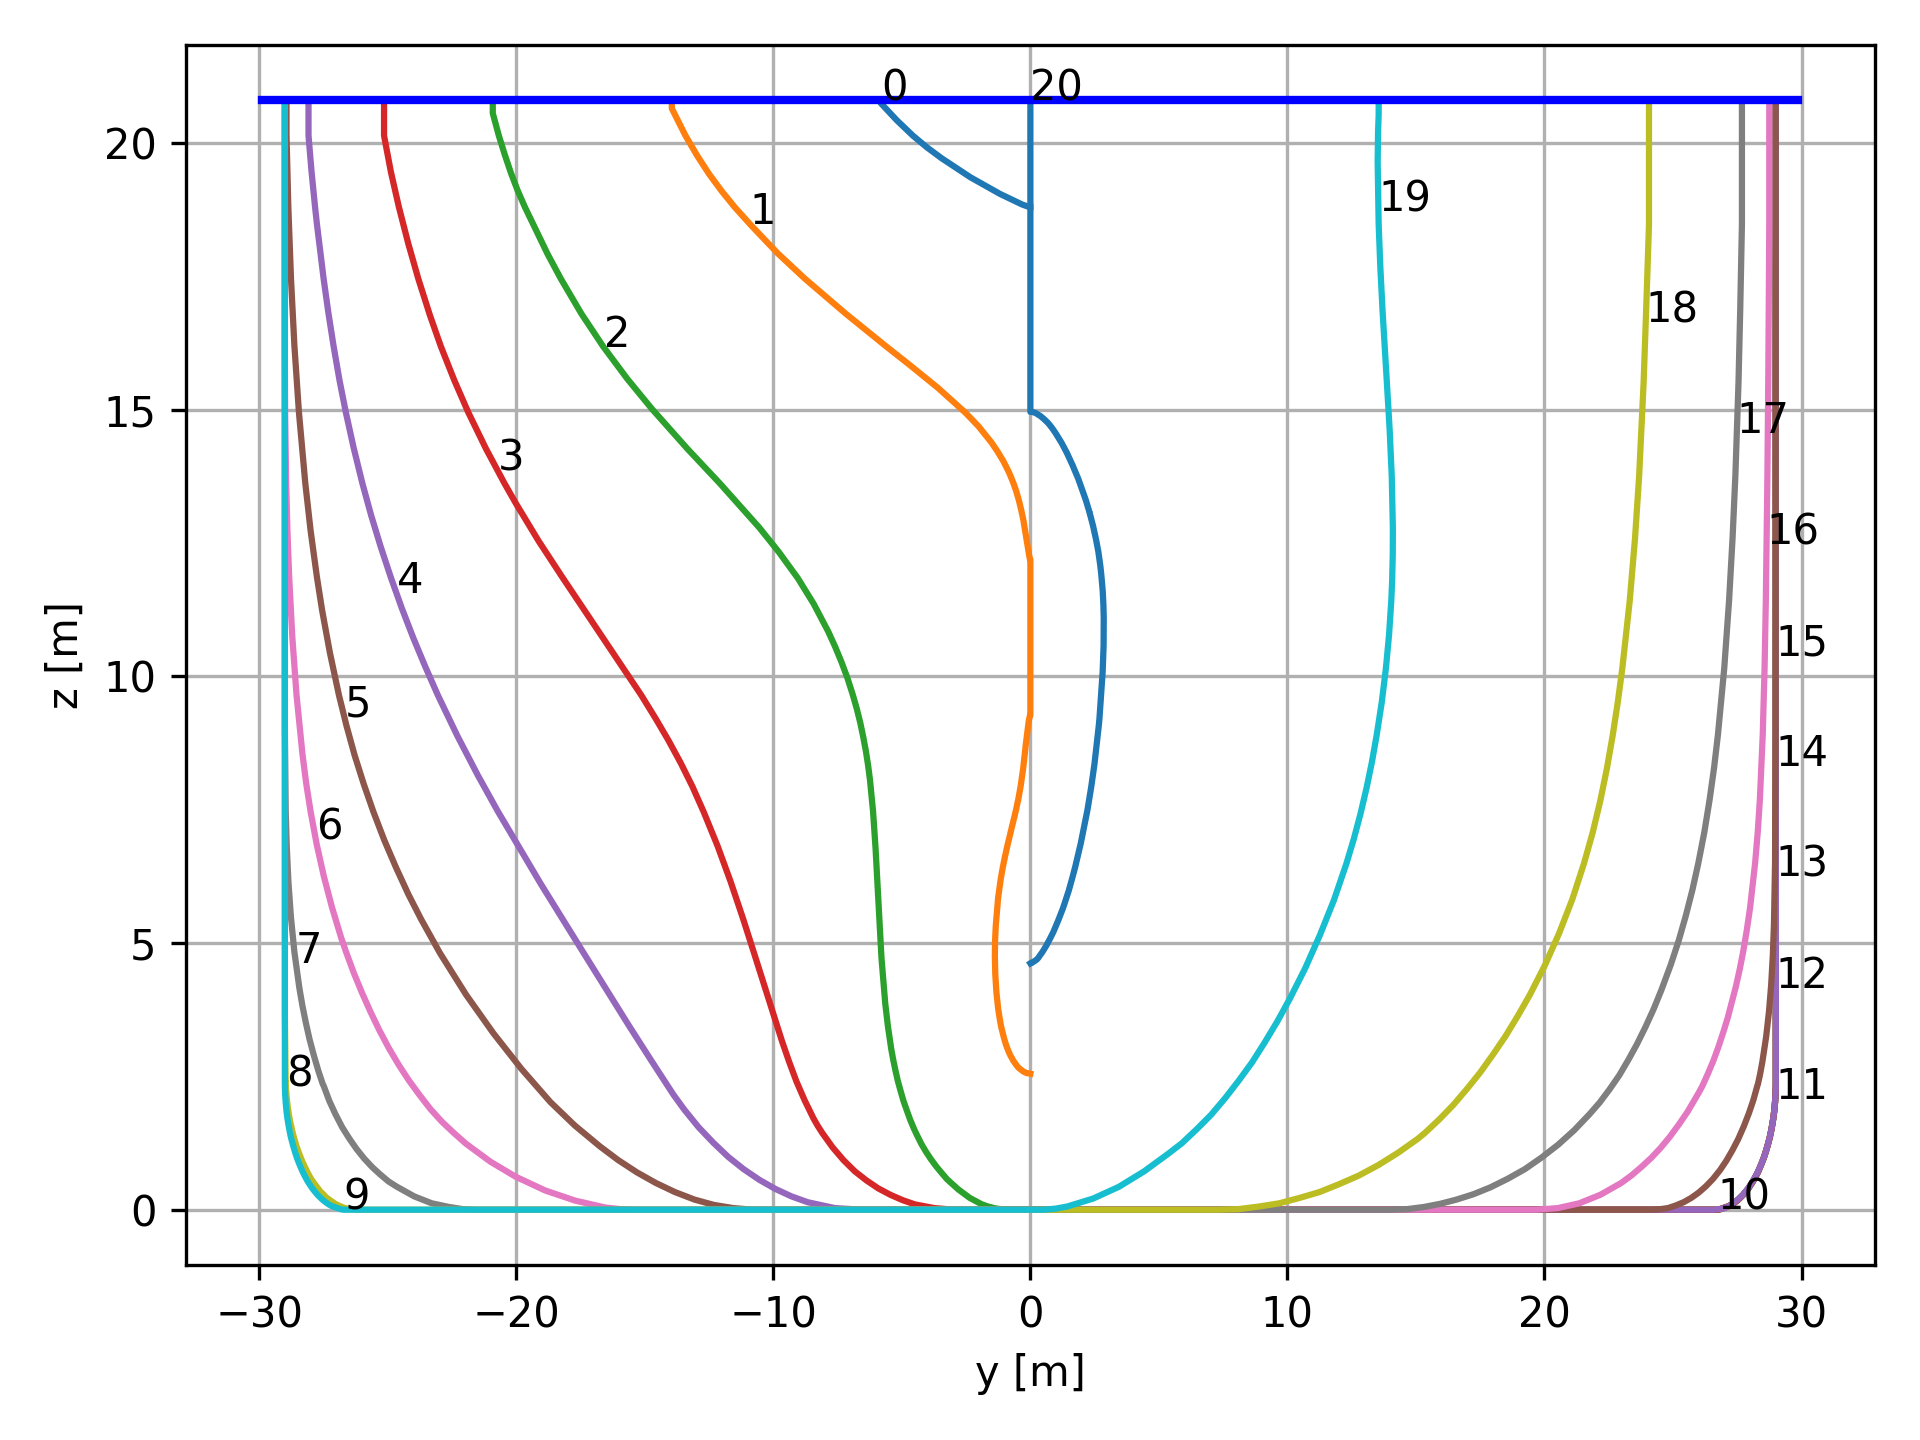
\includegraphics{../figures/KVLCC2_body_plan.png}
\caption{Body plan}
\end{figure}

This ship was selected partly because it is a well known test case and
also because it does not have any bilge keels. The Ikeda's metod contain
methods to predict damping from various components, where the bilge
keels is one of them. Results from roll decay test simulations made with
the Hybrid method will be compared to corresponding model test data from
the SSPA Maritime Dynamics Laboratory. From these model tests, only the
total damping can be observed. Reducing the number of components by
having no bilge keels will therefore give more insight into the
remaining components.

Revisiting an older semi-empirical method such as the Ikeda's method can
also be used to gain a deeper understand of the roll damping
hydrodynamics.
 
            
    
    \begin{longtable}[c]{@{}llllllllll@{}}
\toprule\addlinespace
title & LPP & B & ZCG & KXX & S & V & dens & ta & tf\\\addlinespace 
\midrule\endhead
KVLCC2 & 4.706 & 0.853 & 0.274 & 0.341 & 5.981 & 0.993 & 1000.0 & 0.3059 & 0.3059\\\addlinespace 
\bottomrule 
 \end{longtable}

    

    \section{Typical methods for roll
damping}\label{typical-methods-for-roll-damping}

    \subsection{Roll decay test}\label{roll-decay-test}

The most common way to determine the roll damping of a ship is to
conduct a roll decay test. The initial heel angle during this test gives
the ship potential energy that is shifting to kinetic energy as the ship
starts to move during the inital phase of the roll decay test. The
energy is transfered between kinetic and potential energy during the
oscillations. The ship loses energy over time due to the damping wich
can be seen in this
\href{../../notebooks/02.2_ikeda_Be_assumption.ipynb\#energy}{plot}
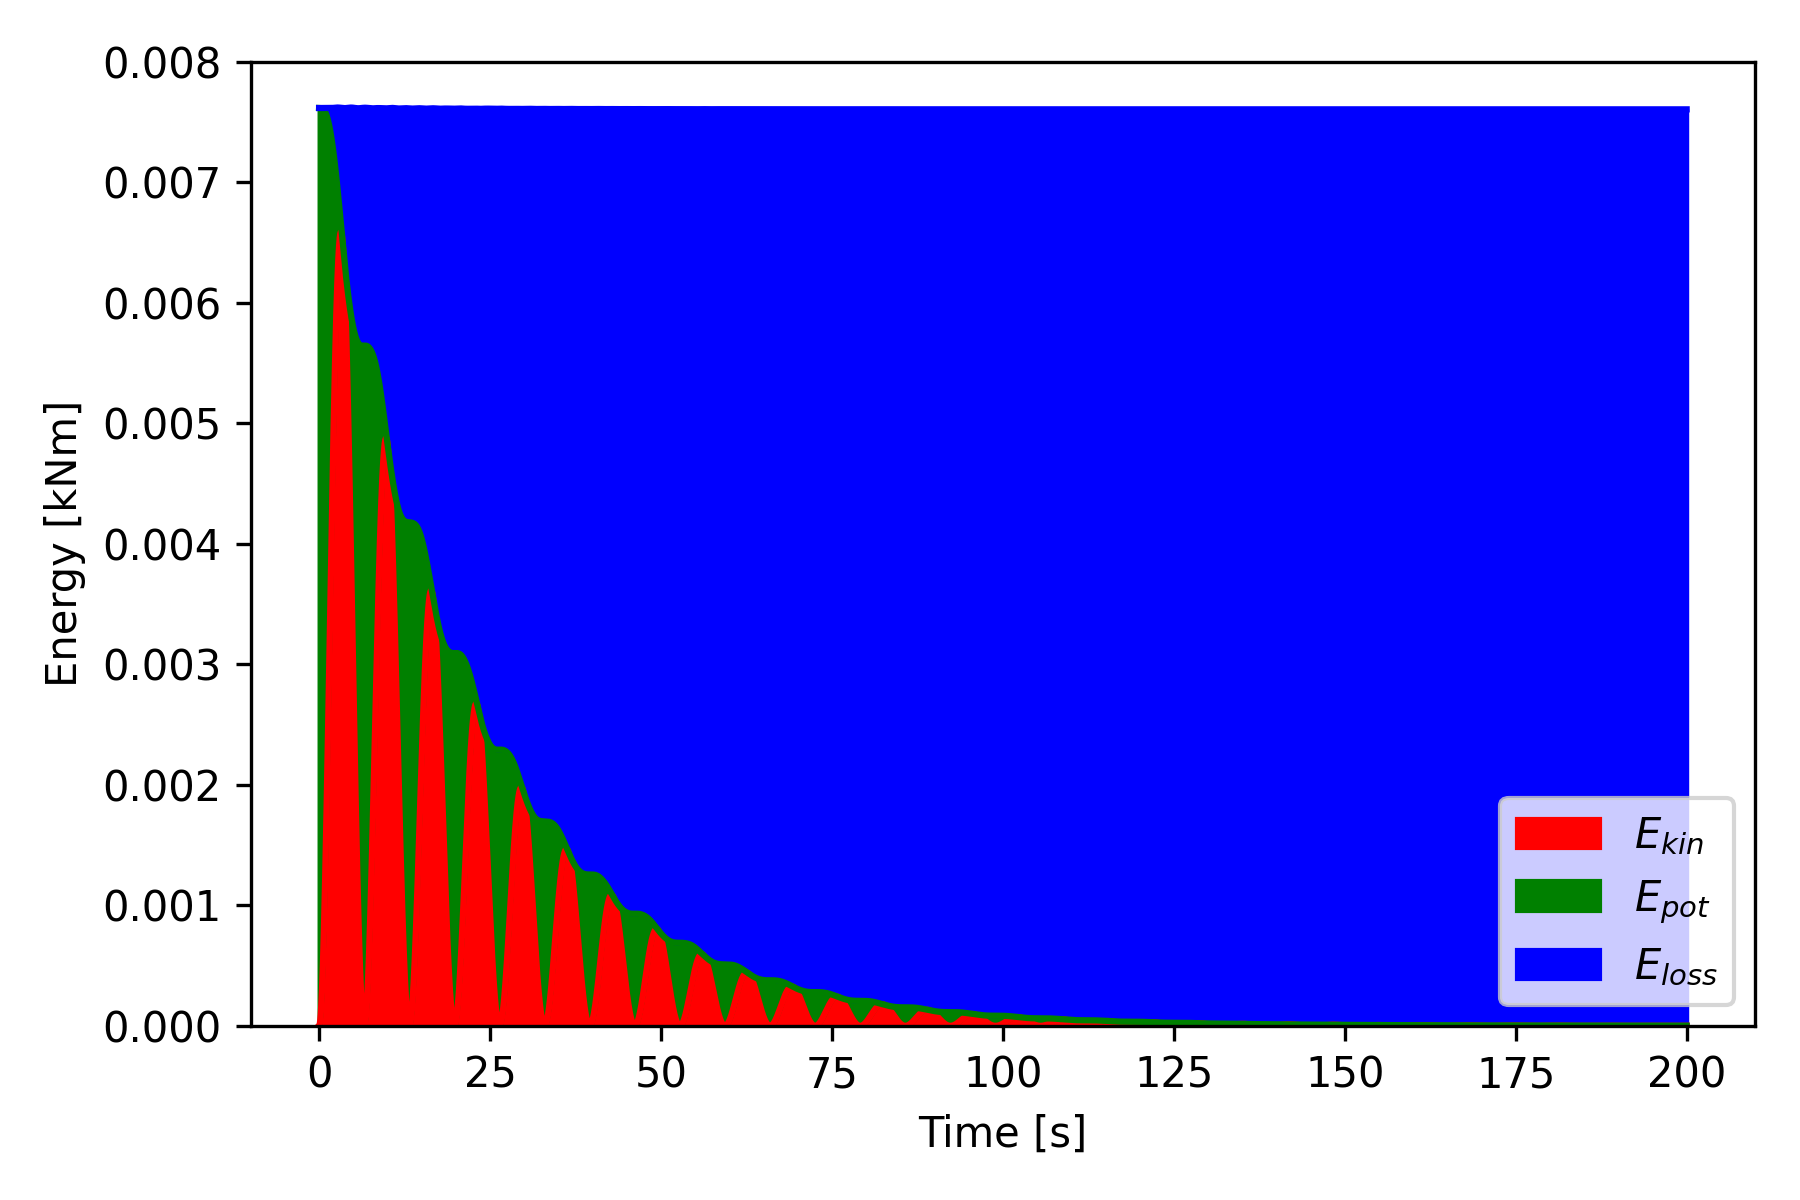
\includegraphics{../figures/energy_transfer.png} Roll decay tests in
model scale experiments as well as from FNPF simulations are used in
this paper to determine the roll damping of KVLCC2. Two different
techniques to identidy the damping from these tests are used: the PIT
method and the logartithmic decrement method which are both described
below.

\subsection{Ikeda's method}\label{ikedas-method}

As a cheaper option to do model tests Ikeda's method can be used to
predict the roll damping. In this method the damping is divided in
various components. This feature enables the possiblity to combine
Ikeda's method with a potential flow method. Ikeda's method is combined
with FNPF giving the Hybrid method as proposed in this paper.

    \subsection{PIT method}\label{pit-method}

    A parameters identification technique (PIT) similar to
\cite{7505983/EXYJELCU} is used to obtain the damping coefficients from
the roll decay model test as well as from the FNPF simulated roll decay
tests. In this technique, parameters in a mathematical model are
determined to get the best fit to a roll decay time signal. A derivation
of a matematical model suitable for this study is described below
together with a description of how the parameters: damping, stiffness
and inertia coefficients are determined.

A differential equation for a linearly decaying motion can be written
as:
 
            
    
    $\displaystyle 
\begin{equation}
\omega_{0}^{2} y + 2 \omega_{0} \zeta \dot{y} + \ddot{y} = 0
\label{eq:equation}
\end{equation}
$

    

    Which has an analytical solution \cite{undefined}:
 
            
    
    $\displaystyle 
\begin{equation}
\phi = \left(\left(\frac{\zeta \phi_{0}}{\sqrt{1 - \zeta^{2}}} + \frac{\dot{\phi}_{0}}{\omega_{0} \sqrt{1 - \zeta^{2}}}\right) \operatorname{sin}\left(\omega_{0} t \sqrt{1 - \zeta^{2}}\right) + \phi_{0} \operatorname{cos}\left(\omega_{0} t \sqrt{1 - \zeta^{2}}\right)\right) e^{- \omega_{0} t \zeta}
\label{eq:equation}
\end{equation}
$

    

    In the usual case of having no initial roll velocity (\(\phi_0=0\)) this
equation can be simlified to:
 
            
    
    $\displaystyle 
\begin{equation}
\phi = \frac{\left(\zeta \operatorname{sin}\left(\omega_{0} t \sqrt{1 - \zeta^{2}}\right) + \sqrt{1 - \zeta^{2}} \operatorname{cos}\left(\omega_{0} t \sqrt{1 - \zeta^{2}}\right)\right) \phi_{0} e^{- \omega_{0} t \zeta}}{\sqrt{1 - \zeta^{2}}}
\label{eq:equation}
\end{equation}
$

    

    And the damping coefficient \(\zeta\) is very small for ships so that
\(\sqrt{1-\zeta}\) is almost 1 and the solution can be further
simplified, into something that can easily be recognized as a decaying
oscillation:
 
            
    
    $\displaystyle 
\begin{equation}
\phi = \phi_{0} e^{- \omega_{0} t \zeta} \operatorname{cos}\left(\omega_{0} t\right)
\label{eq:equation}
\end{equation}
$

    

    The equations derived above are the linear special case of a more
generall expression that can be expressed in general form according to
\cite{7505983/FB64RGPF}:
 
            
    
    $\displaystyle 
\begin{equation}
A_{44} \ddot{\phi} + \operatorname{B_{44}}\left(\dot{\phi}\right) + \operatorname{C_{44}}\left(\phi\right) = 0
\label{eq:equation}
\end{equation}
$

    

    Where \(B_{44}(\dot{\phi})\) and \(C_{44}(\phi)\) are the damping and
stiffness models. A cubic model can be obtained by using cubic damping
and stiffness models:
 
            
    
    $\displaystyle 
\begin{equation}
\operatorname{B_{44}}\left(\dot{\phi}\right) = B_{1} \dot{\phi} + B_{2} \left|{\dot{\phi}}\right| \dot{\phi} + B_{3} \dot{\phi}^{3}
\label{eq:equation}
\end{equation}
$

    
 
            
    
    $\displaystyle 
\begin{equation}
\operatorname{C_{44}}\left(\phi\right) = C_{1} \phi + C_{3} \phi^{3} + C_{5} \phi^{5}
\label{eq:equation}
\end{equation}
$

    

    The total equation is then written:
 
            
    
    $\displaystyle 
\begin{equation}
A_{44} \ddot{\phi} + \left(B_{1} + B_{2} \left|{\dot{\phi}}\right| + B_{3} \dot{\phi}^{2}\right) \dot{\phi} + \left(C_{1} + C_{3} \phi^{2} + C_{5} \phi^{4}\right) \phi = 0
\label{eq:equation}
\end{equation}
$

    

    This mathematical model can be reduced to a quadratic damping model when
\(B_3=0\) and a linear model when \(B_2=B_3=0\). This equation does not
have one unique solutionm however. If all parameters would be multiplied
by a factor \(k\) these parameters would also yield as a solution to the
equation. All parameters are therefore divided by the total added mass
parameters \(A_{44}\), replacing the parameters with new parameters such
as:
 
            
    
    $\displaystyle 
\begin{equation}
B_{1A} = \frac{B_{1}}{A_{44}}
\label{eq:equation}
\end{equation}
$

    

    The equation is now rewritten with these new parameters which have
unique solutions:
 
            
    
    $\displaystyle 
\begin{equation}
\left(B_{1A} + B_{2A} \left|{\dot{\phi}}\right| + B_{3A} \dot{\phi}^{2}\right) \dot{\phi} + \left(C_{1A} + C_{3A} \phi^{2} + C_{5A} \phi^{4}\right) \phi + \ddot{\phi} = 0
\label{eq:equation}
\end{equation}
$

    

    The parameters of this equation can be identified using least square fit
if the time signals \(\phi(t)\), \(\dot{\phi}(t)\) and
\(\ddot{\phi}(t)\) are all known. This is the case for the results from
the FNPF simulations but not from the model tests, where only the roll
signal \(\phi(t)\) is known. The other time derivatives can be estimated
using numerical derivation of a low pass filtered roll signal or Kalman
filtered roll signal. The filtering will however introduce some errors
in itself. So instead of using this "Derivation approach", it has been
found that solving the differential equation numerically for guessed
parameter values determined using optimization similarly to what was
used by \cite{7505983/FJHQJJUH} and \cite{7505983/9B7QMVJJ} gives the
best parameter estimation. One problem with this "Integration approach"
is that in order to converge, the optimization needs a resonable first
guess of the parameters. The Derivation approach has therefore been used
as a pre-step to obtain a very good first guess of the parameters that
can be passed on to the Integration approach. This has been used for
both signals from FNPF and model tests where in the latter case
numerical derivation is used.

The differential equation is numerically solved as an intial value
problem, where the initial states for \(\phi(t)\), \(\dot{\phi}(t)\) and
\(\ddot{\phi}(t)\) are used to estimate the following states, by
conducting very small time steps using the follownig expression for the
acceleration:
 
            
    
    $\displaystyle 
\begin{equation}
\ddot{\phi} = - B_{1A} \dot{\phi} - B_{2A} \left|{\dot{\phi}}\right| \dot{\phi} - B_{3A} \dot{\phi}^{3} - C_{1A} \phi - C_{3A} \phi^{3} - C_{5A} \phi^{5}
\label{eq:equation}
\end{equation}
$

    

    This numerical solution can be compared with the analytical solution
above for a linear model. For this case the relation between \(\zeta\)
and \(B_1\) can be expressed as:
 
            
    
    $\displaystyle 
\begin{equation}
B_{1} = 2 A_{44} \omega_{0} \zeta
\label{eq:equation}
\end{equation}
$

    

    and the natural frequency can be obtained from:
 
            
    
    $\displaystyle 
\begin{equation}
\omega_{0} = \sqrt{\frac{C_{1}}{A_{44}}}
\label{eq:equation}
\end{equation}
$

    

    The analytical and numerical solutions are vary similar according to the
example: \(A_{44} = 1.0\), \(B_1 = 0.3\), \(C_1 = 5.0\) shown in the
figure below.

    \begin{Verbatim}[commandchars=\\\{\}]
findfont: Font family ['"serif"'] not found. Falling back to DejaVu Sans.
    \end{Verbatim}

    \begin{center}
    \adjustimage{max size={0.9\linewidth}{0.9\paperheight}}{output_37_1.pdf}
    \end{center}
    { \hspace*{\fill} \\}
    
    \section{Sensitivity analysis of Ikeda's
method}\label{sensitivity-analysis-of-ikedas-method}

Ikeda's method divides roll damping into five damping components:

\begin{longtable}[]{@{}ll@{}}
\toprule
Symbol & Component\tabularnewline
\midrule
\endhead
\(B_F\) & skin friction\tabularnewline
\(B_E\) & eddy generation\tabularnewline
\(B_L\) & hull lift\tabularnewline
\(B_W\) & roll wave generation\tabularnewline
\(B_{BK}\) & bilge keels\tabularnewline
\bottomrule
\end{longtable}

And the total damping is written as the sum of these components,

\begin{equation}
B_{44} = B_F + B_E + B_L + B_W + B_{BK}
\end{equation}

Due to the absence of bilge keels for the KVLCC2 the \(B_{BK}\) does not
need to be included. This means that remaining components will get all
the attention in this paper. Ikeda has in a series of papers proposed
semi empirical formulas for the viscous damping components: \(B_F\),
\(B_E\) and \(B_L\) which have been implemented for this study. The wave
damping \(B_W\) is calculated using a potential flow strip theory code
or a more advance potential flow code such as the FNPF method later
described as the Hybrid method in this paper.

Ikeda produced many papers about various aspects of roll damping where
most of them are translations from original manuscripts in Japanese.
Summaries of this method \cite{7505983/FB64RGPF},
\cite{7505983/KAKIM2E2} and \cite{7505983/UGK6YEVD} has been used
together with the original papers to understand how the method should be
implemented. Falzarano says that the Himeno report and associated
computer programs are well-known to have numerous typographical errors.
When looking at these resources it becomes evident that there is some
variety on how the method should be implemented, regardless if this is
due to typographical errors or being variations of the actual method.
The implementation was therefore a fairly time consuming task where
various alternative implementations needed to be compared and
investigated.

The scale effects of roll damping is considered to mainly be associated
with the sking friction component \(B_F\) \cite{7505983/FB64RGPF}. This
component makes a very small part of the total damping for the full
scale ship, but a substantial part for the model scale ship used in this
study. This is therefore the only component in ikedas method that needs
to be recalculated when the scale changes.

For the skin friction damping \(B_F\) implementation was made according
to the description in \cite{7505983/UGK6YEVD}. With the difference that
the actual wetted surface \(S\) was used instead of the proposed
estimation formula.

The hull lift damping \(B_L\) is calculated according to
\cite{7505983/937PN5DT} and implemented as described in
\cite{7505983/UYUAYY7E}. Journe added a linear interpolation to the
values for \(\kappa\) from the Ikeda paper.

A schematic graph of how the parameters vary with speed and roll angle
amplitude \(\phi_a\) in the current model scale is created with the
current implementation of Ikeda as shown below. The roll amplitude is
first varied at zero speed (left). The speed is then varied from zero to
the froude number corresponding to 15.5 knots in full scale for the
KVLCC2 with a roll angle amplitude of 10 degrees (middle). The amplitude
is then gradually reduced at the highest froude number down to zero
again (right).

Assumming that the trends are correct in Ikeda's method it can be noted
from the amplitude variations at zero knots (left): * \(B_W\) does not
change with amplitude, implying that they only contribute to the linear
part (\(B_1\)) of the damping. (The \(B_W\) was calculated with strip
theory here) * \(B_F\) has a small amplitude dependancy but the linear
part is dominating. * \(B_E\) has a large amplitude depandancy and only
contributes to the quadratic damping (\(B_2\))\cite{7505983/4AFVVGNT}.

Looking at the speed variation (middle): * At low speed \(B_F\) and
\(B_E\) are the dominating components. (Note that this ship does not
have bilge keels, as that would otherwise also be a large component). *
At high speed the \(B_E\) has almost disappeared and is replaced by the
\(B_L\) which is now the dominating component. * \(B_F\) has a large
contribution for all speeds (at model scale).

Looking at the roll amplitude variation (right): * (Please note that
this x-axis is revered in this graph) * \(B_L\) does not change with
amplitude, implying that they only contribute to the linear part
(\(B_1\)) of the damping. * \(B_F\) has a small amplitude dependancy but
the linear part is dominating.

    \begin{center}
    \adjustimage{max size={0.9\linewidth}{0.9\paperheight}}{output_39_0.pdf}
    \end{center}
    { \hspace*{\fill} \\}
    
    When the damping predicted with Ikeda was compared with corresponding
model test it was found that the results were in poor agreement for the
zero speed case but quite good results at speed. This was pointing
towards the eddy damping being incorrect in the current implementation
of Ikeda's method. A thurough investigation of the eddy damping
prediction was therefore conducted which is described in the next
section.

    \subsection{Eddy damping}\label{eddy-damping}

The eddy damping is due to eddies generated around the ship hull during
the roll motion. Strong eddies occures at sharp edges in the geometry.
Below is an illustration of how the eddy damping changes with bilge
radius to beam ratio as predicted with the current implementation of the
method. It seems that the damping approaches zero very fast as the bilge
radius increase. So having just a small rounding of the bilge, compared
to a square section, will have a great impact on the eddy roll damping.

    \begin{center}
    \adjustimage{max size={0.9\linewidth}{0.9\paperheight}}{output_42_0.pdf}
    \end{center}
    { \hspace*{\fill} \\}
    
    Ikeda made experiements on a number of two-dimensional cylinders with
various sections \cite{7505983/4AFVVGNT}. Ikeda found that the eddy
damping per unit length of these sections can be expressed as:
 
            
    
    $\displaystyle 
\begin{equation}
B'_{E0} = \frac{4 C_{r} T_{s}^{4} \omega \phi_{a} \rho}{3 \pi}
\label{eq:equation}
\end{equation}
$

    

    The total eddy damping can be obtained as an integral over the sections
along the ship hull:
 
            
    
    $\displaystyle 
\begin{equation}
B_{E0} = \int\limits_{AP}^{FP} B'_{E0}\, dx
\label{eq:equation}
\end{equation}
$

    

    It can be seen from the section damping equation above that the eddy
damping increases linearly with both roll amplitude and frequency, and
that it will go to zero for small amplitudes and frequencies, which
means that it is only included in the quadratic damping term (\(B_2\)).
Ikeda expressed the \(C_r\) coefficient to be entirely depending on the
hull form. Ikeda developed a regression formula for \(C_r\) based on his
experiments, which is used in the prediction method. The authors of this
paper have tried to implement this method according to the description
in the original paper \cite{7505983/4AFVVGNT} but have failed to
reproduce the results from Ikeda's experiments exactly. Other resources
such as \cite{7505983/FB64RGPF} and \cite{7505983/KAKIM2E2} have also
been used without success.

Instead a new regression for \(C_r\) was made on the experimental
results from \cite{7505983/4AFVVGNT}. The experimental results (below)
were collected by the authors using manual digitalization.
 
            
    
    \begin{longtable}[c]{@{}lllllllllllll@{}}
\toprule\addlinespace
model & $\hat{\omega}$ & $\phi_a$ & $\hat{B_E}^*$ & B_W+B_F & $L_{pp}$ & $beam$ & $T_s$ & $\sigma$ & $R_b$ & $a_1$ & $a_3$ & $C_r$\\\addlinespace 
\midrule\endhead
A & 0.7509999999999999 & 0.23 & 0.03753367571367666 & 0.0036357630291343353 & 0.8 & 0.28 & 0.11199999999999999 & 1.0 & 0.0 & 0.09572067327729883 & -0.13851394050431068 & 6.791066236924095\\\addlinespace 
A & 0.507 & 0.24 & 0.028412505258521625 & 0.001390847207830892 & 0.8 & 0.28 & 0.11199999999999999 & 1.0 & 0.0 & 0.09572067327729883 & -0.13851394050431068 & 7.297514558176523\\\addlinespace 
B & 0.7509999999999999 & 0.3 & 0.02070022681130489 & 0.003265431521957657 & 0.8 & 0.28 & 0.11199999999999999 & 0.997 & 0.01 & 0.09594956148239993 & -0.13645394665840074 & 2.862276498613116\\\addlinespace 
B & 0.536 & 0.3 & 0.013327670129715686 & 0.0011106958095124797 & 0.8 & 0.28 & 0.11199999999999999 & 0.997 & 0.01 & 0.09594956148239993 & -0.13645394665840074 & 2.5820572246775715\\\addlinespace 
C & 0.7509999999999999 & 0.27 & 0.006150584844546503 & 0.0021146614051981705 & 0.8 & 0.28 & 0.11199999999999999 & 0.995 & 0.02 & 0.09610173289389044 & -0.13508440395498614 & 0.942686403519787\\\addlinespace 
C & 0.625 & 0.21 & 0.003986684713683185 & 0.0015000392814414284 & 0.8 & 0.28 & 0.11199999999999999 & 0.995 & 0.02 & 0.09610173289389044 & -0.13508440395498614 & 0.9439893821974789\\\addlinespace 
D & 0.939 & 0.31 & 0.007465704560231518 & 0.0020385726488099023 & 0.8 & 0.28 & 0.11199999999999999 & 0.988 & 0.03 & 0.09663180060654622 & -0.13031379454108408 & 0.7906835390460057\\\addlinespace 
D & 0.7509999999999999 & 0.31 & 0.006144708627086015 & 0.0015002944963602304 & 0.8 & 0.28 & 0.11199999999999999 & 0.988 & 0.03 & 0.09663180060654622 & -0.13031379454108408 & 0.8136897536952459\\\addlinespace 
G & 0.8140000000000001 & 0.24 & 0.011504995055307304 & 0.08835564931140577 & 0.8 & 0.185 & 0.192 & 0.799 & 0.18239704162959489 & -0.3470782119390985 & -0.007600489480668136 & 0.08606062205238546\\\addlinespace 
H & 0.56 & 0.3 & 0.0006398363737784848 & 0.0014000371877776175 & 0.8 & 0.39799999999999996 & 0.193 & 0.893 & 0.19570204423684776 & 0.014252111702710376 & -0.0688620354229256 & 0.0596772641355714\\\addlinespace 
H & 0.889 & 0.3 & 0.0011242278371175344 & 0.002290023345660393 & 0.8 & 0.39799999999999996 & 0.193 & 0.893 & 0.19570204423684776 & 0.014252111702710376 & -0.0688620354229256 & 0.0660511799369215\\\addlinespace 
I & 0.58 & 0.25 & 0.0017690750019860046 & 0.0009999925056469947 & 0.8 & 0.237 & 0.096 & 0.977 & 0.0493806713819148 & 0.09198685657943263 & -0.12305863394274225 & 0.3580373791465449\\\addlinespace 
I & 0.861 & 0.25 & 0.001950180538963892 & 0.00250475666585228 & 0.8 & 0.237 & 0.096 & 0.977 & 0.0493806713819148 & 0.09198685657943263 & -0.12305863394274225 & 0.2658776209301261\\\addlinespace 
J & 1.03 & 0.23 & 0.004696651608905555 & 0.002761633629519946 & 0.8 & 0.34299999999999997 & 0.192 & 0.593 & 0.3534094529483184 & -0.06336616200212129 & 0.12359023842785882 & 0.13572061257096327\\\addlinespace 
K & 0.78 & 0.29 & 0.017659813274832913 & 0.0013035049232182035 & 1.0 & 0.193 & 0.125 & 0.541 & 0.22715551565933745 & -0.14872060747212207 & 0.1558461247394752 & 0.29254752963292663\\\addlinespace 
L & 0.551 & 0.26 & 0.1342976216222535 & 0.02880233570839885 & 1.0 & 0.151 & 0.14400000000000002 & 0.43 & 0.240320284977418 & -0.37779280539751503 & 0.21059154430298574 & 0.9275961561025332\\\addlinespace 
\bottomrule 
 \end{longtable}

    

    Where \(OG/d=0\) for all sections. For the Series60 sections (G-K) the
bilge radius \(R_b\) was estimated using the following estimation,
proposed by the authors:
 
            
    
    $\displaystyle 
\begin{equation}
R_{b} = \frac{\sqrt{B_{s} T_{s} \left(1 - \sigma\right)}}{\sqrt{1 - \frac{\pi}{4}}}
\label{eq:equation}
\end{equation}
$

    

    The nondimensional damping is expressed in \cite{7505983/4AFVVGNT} using
a star (*) sign. The reason seams to be that Ikeda wanted to signal that
this damping only has the quadratic part of the damping. This stared
damping are defined as:
 
            
    
    $\displaystyle 
\begin{equation}
B_{E0 HAT} = \frac{8 B_{E star hat}}{3 \pi}
\label{eq:equation}
\end{equation}
$

    

    \(\hat{B_E}^*\) and \((B_W+B_F)^*\) are the experimental values taken
from \cite{7505983/4AFVVGNT}. Which add up to the total damping:

    \(\hat{B^*} = \hat{B^*_E} + (B_W+B_F)^*\)

    The Lewis section coefficients were calculated as:
 
            
    
    $\displaystyle 
\begin{equation}
D_{1} = \frac{4 \sigma}{\pi} + \frac{\left(H_{0} - 1\right)^{2} \left(- \frac{4 \sigma}{\pi} + 1\right)}{\left(H_{0} + 1\right)^{2}} + 3
\label{eq:equation}
\end{equation}
$

    
 
            
    
    $\displaystyle 
\begin{equation}
a_{3} = \frac{- D_{1} + \sqrt{9 - 2 D_{1}} + 3}{D_{1}}
\label{eq:equation}
\end{equation}
$

    
 
            
    
    $\displaystyle 
\begin{equation}
a_{1} = \frac{\left(H_{0} - 1\right) \left(a_{3} + 1\right)}{H_{0} + 1}
\label{eq:equation}
\end{equation}
$

    
 
            
    
    $\displaystyle 
\begin{equation}
B_{E0 HAT} = \frac{8 B_{E star hat}}{3 \pi}
\label{eq:equation}
\end{equation}
$

    

    And the \(C_r\) was calculated from the experiments as:
 
            
    
    $\displaystyle 
\begin{equation}
C_{r} = \frac{3 \pi B_{E0 HAT} B_{s} T_{s} beam^{2} \sigma}{4 T^{4} \omega_{hat} \phi_{a}}
\label{eq:equation}
\end{equation}
$

    

    Instead of trying to invent some very advanced mathematical expression
for the \(C_r\) regression a simple decision tree model was instead
fitted to the \(C_r\) data from Ikeda's experiments. The fitted decision
tree is illustrated in the figure below:

    \begin{center}
    \adjustimage{max size={0.9\linewidth}{0.9\paperheight}}{output_63_0.pdf}
    \end{center}
    { \hspace*{\fill} \\}
    
    Eventhoug this tree is so simple it has very good accuracy in
reproducing the results from Ikedas experiments (\(r^2=0.996)\). The
\(C_r\) was predicted with Ikeda and the alternative decision tree model
for the KVLCC2 with section data according to the table below. A
comparison is shown in the figure below, where it can be seen that the
Ikeda implementation predicts much higher \(C_r\) between station 8 and
14, where the bilge radius is also very small.
 
            
    
    \begin{longtable}[c]{@{}llllllll@{}}
\toprule\addlinespace
$x$ & $beam$ & $T_s$ & $\sigma$ & $\frac{OG}{d}$ & $R_b$ & $a_1$ & $a_3$\\\addlinespace 
\midrule\endhead
-0.08080882352941177 & 0.17115554117647058 & 0.029411764705882353 & 0.5939992517452843 & 1.0999999999999996 & 0.09758941694170616 & 0.5340949013902127 & 0.09346077843706034\\\addlinespace 
0.14941076470588238 & 0.4101988529411765 & 0.26838235294117646 & 0.2432956630457875 & 0.12054794520547941 & 0.6230466900619334 & -0.1824458277260031 & 0.3650565796464702\\\addlinespace 
0.4125188823529412 & 0.6150630000000001 & 0.3058823529411765 & 0.49222807909482774 & 0.10576923076923073 & 0.6671978461991239 & 0.003203556976734904 & 0.19158944479904777\\\addlinespace 
0.6427384705882353 & 0.7394487352941176 & 0.3058823529411765 & 0.653718963842786 & 0.10576923076923073 & 0.6041278867085014 & 0.10239362220051965 & 0.08357826147472612\\\addlinespace 
0.9058465882352942 & 0.8258710588235294 & 0.3058823529411765 & 0.7857936964338019 & 0.10576923076923073 & 0.5021491605629501 & 0.14889281493367498 & -0.00024621915261740444\\\addlinespace 
1.1360661764705882 & 0.8510367352941176 & 0.3058823529411765 & 0.8780056081159271 & 0.10576923076923073 & 0.38468440514364793 & 0.15415047011882232 & -0.057593441230048115\\\addlinespace 
1.3662857647058824 & 0.8529412941176471 & 0.3058823529411765 & 0.9445485696925716 & 0.10576923076923073 & 0.25964289371087323 & 0.14822611734831342 & -0.09979784926318554\\\addlinespace 
1.6293938235294119 & 0.8529412941176471 & 0.3058823529411765 & 0.9837969411523451 & 0.10576923076923073 & 0.1403519881372493 & 0.1440002403931892 & -0.12546231104499617\\\addlinespace 
1.8596135294117646 & 0.8529412941176471 & 0.3058823529411765 & 0.9973617422737119 & 0.10576923076923073 & 0.05663418741256937 & 0.14250677906686124 & -0.134532352965095\\\addlinespace 
2.1227216176470587 & 0.8529412941176471 & 0.3058823529411765 & 0.9979523911561022 & 0.10576923076923073 & 0.04989345314050447 & 0.14244128456104196 & -0.13493011211884393\\\addlinespace 
2.3529411764705883 & 0.8529412941176471 & 0.3058823529411765 & 0.9979517810766112 & 0.10576923076923073 & 0.04990088539633636 & 0.14244135223122248 & -0.13492970114645178\\\addlinespace 
2.5866385294117644 & 0.8529412941176471 & 0.3058823529411765 & 0.9979512935186544 & 0.10576923076923073 & 0.049906824245393284 & 0.1424414063112502 & -0.13492937270934396\\\addlinespace 
2.853721176470588 & 0.8529412941176471 & 0.3058823529411765 & 0.9979517810766112 & 0.10576923076923073 & 0.04990088539633636 & 0.14244135223122248 & -0.13492970114645178\\\addlinespace 
3.087418529411765 & 0.8529412941176471 & 0.3058823529411765 & 0.9979517810766112 & 0.10576923076923073 & 0.04990088539633636 & 0.14244135223122248 & -0.13492970114645178\\\addlinespace 
3.3211158823529408 & 0.8529412941176471 & 0.3058823529411765 & 0.9979326878514596 & 0.10576923076923073 & 0.05013293059480477 & 0.14244347003477187 & -0.13491683936916107\\\addlinespace 
3.588198529411765 & 0.8527555294117647 & 0.3058823529411765 & 0.9912384299601698 & 0.10576923076923073 & 0.10319620688499365 & 0.14309046599982314 & -0.13042795627929626\\\addlinespace 
3.821895882352942 & 0.8454087058823531 & 0.3058823529411765 & 0.9700959804598432 & 0.10576923076923073 & 0.1898272847533075 & 0.14164643465147272 & -0.11659011810535287\\\addlinespace 
4.0555932352941175 & 0.8141369117647059 & 0.3058823529411765 & 0.9357906856132224 & 0.10576923076923073 & 0.2729657971444984 & 0.1284632648706989 & -0.09485605304001271\\\addlinespace 
4.2892905882352945 & 0.7078072941176471 & 0.3058823529411765 & 0.8981468043116771 & 0.10576923076923073 & 0.32055705586758354 & 0.0675552738224847 & -0.07182793147878982\\\addlinespace 
4.556373235294117 & 0.41476041176470585 & 0.3058823529411765 & 0.8566227195636964 & 0.10576923076923073 & 0.2911382798056208 & -0.18351472793269105 & -0.043764611706507486\\\addlinespace 
4.790070588235294 & 0.08396374705882353 & 0.23794117647058824 & 0.47076332581694846 & 0.1359703337453646 & 0.22196727820657103 & -0.7721801546355255 & 0.1030403802769838\\\addlinespace 
\bottomrule 
 \end{longtable}

    

    \begin{center}
    \adjustimage{max size={0.9\linewidth}{0.9\paperheight}}{output_66_0.pdf}
    \end{center}
    { \hspace*{\fill} \\}
    
    These two alternative ways to calculate the eddy damping will be further
discussed below, when comparing the total predicted damping with
corresponding results from the model tests.

    \subsection{Time and frequency domain}\label{time-and-frequency-domain}

Ikeda's method is defined in the frequency domain, where the damping is
expressed as a function of roll angle amplitude \(\phi_a\) and roll
angle frequency \(\omega\). The equivalent linear damping \(B_e\) (not
to confuse with eddy damping \(B_E\)) is a way to convert the frequency
domain damping into time domain damping \cite{7505983/FB64RGPF}, so that
time domain roll simulations can be conducted with results from Ikeda's
method. The most general way to determine \(B_e\) is to assume that the
energy loss due to damping during a half cycle of roll is the same when
nonlinear and linear dampings are used \cite{7505983/RYUBZITQ}. The
\(B_e\) can then be calculated as a Fourier series expansion of the
damping model, which in the case of a cubic model yields as:
 
            
    
    $\displaystyle 
\begin{equation}
B_{e} = B_{1} + \frac{8 B_{2} \omega_{0} \phi_{a}}{3 \pi} + 0.75 B_{3} \omega_{0}^{2} \phi_{a}^{2}
\label{eq:equation}
\end{equation}
$

    

    In the case of a quadratic model \(B_3=0\) and for the linear model
\(B_1\) and \(B_e\) are the same thing.

    The expression above gives a relation between the frequency domain
quantities \(\phi_a\), \(\omega\) and the time domain quantities
\(B_1\), \(B_2\) and \(B_3\) which can be used to obtain the latter ones
from the Ikeda's method. This can be done by calculating the damping
with Ikeda's method for a variation of frequencies and amplitudes and
then fit the above expression to this damping and obtain \(B_1\),
\(B_2\) and \(B_3\):

\[B^{Ikeda}(\phi_a, \omega) = B_e(\phi_a, \omega)\]

In the case of a roll decay test \(\phi_a\) is the only parameter being
varied. In order to verify this approach, an alternative method using
the logaritmic decrement \cite{7505983/BYNJ8CFG} to obtaining the
frequency domain quantities from time series result is also used.

This method is investigated on simulation results with a quadratic
model: \(B_1 = 0.05\), \(B_2 = 0.9\), \(A_{44} = 1.0\), \(C_1 = 5.0\).
The peak values, being the only known amplitudes from this signal, is
shown in the figure below.

    \begin{center}
    \adjustimage{max size={0.9\linewidth}{0.9\paperheight}}{output_72_0.pdf}
    \end{center}
    { \hspace*{\fill} \\}
    
    The decrement is calculated as the ratio between every other peak, so
that negative and positive roll peaks are separated. This decrement can
be calulated for each peak:
\[ \Delta_n = \frac{\phi_{a,n}}{\phi_{a,n+2}}\]

    The nondimensional \(\zeta\) damping coefficient for each peak can be
calculated from the logaritimic decrement:

    \[\zeta_n = \frac{\delta_n}{2\pi}=\frac{ln(\Delta_n)}{2\pi}\]

    The dimensional damping \(B_n\) (Nm*s) can be then be obtained:
 
            
    
    $\displaystyle 
\begin{equation}
B = 2 A_{44} \omega_{0} \zeta
\label{eq:equation}
\end{equation}
$

    

    So the damping can be obtained for each oscillation this way but it is
not obvious which of the roll amplitudes these dampings correspond to.
Four different choices were tried, associating damping \(B_n\) with the
following amplitudes: * A : \(\phi_n\) * B : \(\phi_{n+1}\) * C :
\(\phi_{n+2}\) * D : \((\phi_n + \phi_{n+1} + \phi_{n+2})/3\)

    \begin{center}
    \adjustimage{max size={0.9\linewidth}{0.9\paperheight}}{output_79_0.pdf}
    \end{center}
    { \hspace*{\fill} \\}
    
    Taking the mean value of peak n and the following two peaks (alt.D) seem
to be the approach that best matches the \(B_e\) (predicted using the
linearized equivalent damping method). The linearized equivalent damping
method therefore seems to be the best way to convert \(B_1\), \(B_2\),
\(B_3\) to frequency domain, considering the difficulties with the
logaritmic decrement method as described above. The only time linearized
equivalent damping method has not been used in this paper, is when
damping at individual peaks from a time signal should be converted to
frequency domain.

    \subsection{Proposed hybrid method}\label{proposed-hybrid-method}

\subsubsection{Proposed model}\label{proposed-model}

A Hybrid method has been developed where wave damping \(B_W\) obtained
with FNPF as described in the previous section is used together with the
visous damping contributions from Ikeda's method. The wave damping was
determined by using the PIT described above on results from FNPF
simulations of roll decay tests.

\subsubsection{FNPF method}\label{fnpf-method}

    \section{Results}\label{results}

    \subsection{Roll decay model tests}\label{roll-decay-model-tests}

\subsubsection{0 knots}\label{knots}

Data from two roll decay model tests conducted at zero speed were
available:
\href{../../notebooks/01.2_select_suitable_MDL_test_KLVCC2.ipynb\#rolldecay}{Roll
decay model tests 0 knots}. These tests where analyzed by fitting a
\href{../../notebooks/01.2_select_suitable_MDL_test_KLVCC2.ipynb\#cubic_model}{Cubic
model} to the model test data. The two models were very similar in terms
of roll damping and stiffness, suggesting good repeatability in the
model tests as well as in the parameter identification technique (PIT)
used. The individual damping from each oscillation obtained with the
logarithmic decrement method are very scattered, but this does not seem
to influence the two models for the 0 speed case, which are very
similiar.

    \subsubsection{15.5 knots}\label{knots}

Data from one roll decay model tests conducted at a ship speed
corresponding to 15.5 knots full scale ship speed was also available.
This model tests was analyzed in the same way as the other tests. It was
found that the damping was higher at speed. The ship got a small
\href{../../notebooks/01.3_select_suitable_MDL_test_KLVCC2_speed.ipynb\#yawrate}{yaw
rate} at the end of test, giving a small steady roll angle due to the
centrifugal force. Since this effect is not included in the matematical
model used, the steady roll angle was instead removed by removing the
linear trend in the roll angle signal.

    \begin{center}
    \adjustimage{max size={0.9\linewidth}{0.9\paperheight}}{output_87_0.pdf}
    \end{center}
    { \hspace*{\fill} \\}
    
    \subsection{Ikeda's method}\label{ikedas-method}

    When looking at predictions for KVLCC2 at 0 speed made with regular
Ikeda's method, it was found that the eddy damping \(B_E\) was too high
compared with the regular implementation, compared to the model test
results. Eventhough the rest of the components would also be
overpredicted, the \(B_E\) would still be too large. The eddy damping
calculated with \(C_r\) predicted with the descision tree gave much
better agreement.

    \begin{center}
    \adjustimage{max size={0.9\linewidth}{0.9\paperheight}}{output_91_0.pdf}
    \end{center}
    { \hspace*{\fill} \\}
    
    \subsection{FNPF}\label{fnpf}

Simulations of roll decay tests were conducted with FNPF for each model
test. The results from these simulations can be seen in the figure
below.

    \begin{center}
    \adjustimage{max size={0.9\linewidth}{0.9\paperheight}}{output_94_0.pdf}
    \end{center}
    { \hspace*{\fill} \\}
    
    \subsection{Roll damping prediction with Hybrid
method}\label{roll-damping-prediction-with-hybrid-method}
Replacing the wave damping $B_W$, for the zero speed case above, with values obtained with FNPF is shown below. 
    \begin{center}
    \adjustimage{max size={0.9\linewidth}{0.9\paperheight}}{output_97_0.pdf}
    \end{center}
    { \hspace*{\fill} \\}
    
    FNPF gave stable results at zero speed, but very unstable results at
speed, due to what was thought to be memory effects. For the speed case
the viscous damping was instead present during the actual FNPF
simulations. The viscous damping was included by adding a linear
\(B_{visc,1}\) and quadratic \(B_{visc,2}\) damping term the equation of
motions in the FNPF. The results are compared with corresponding results
from the model tests.

    \begin{center}
    \adjustimage{max size={0.9\linewidth}{0.9\paperheight}}{output_99_0.pdf}
    \end{center}
    { \hspace*{\fill} \\}
    
    The results using the Hybrid method for Run 3 at speed gives very
similar results to the corresponding model tests.

    \begin{center}
    \adjustimage{max size={0.9\linewidth}{0.9\paperheight}}{output_101_0.pdf}
    \end{center}
    { \hspace*{\fill} \\}
    
    The coefficients obtained from model tests, FNPF and Hybrid method are
summarized in model scale units in the table below:
 
            
    
    \begin{longtable}[c]{@{}lllllll@{}}
\toprule\addlinespace
run & method & $F_n$ & $\omega_0$ & $B_1$ & $B_2$ & $B_3$\\\addlinespace 
\midrule\endhead
1 & model test & 0.0 & 2.461405663797153 & 2.960431148229692 & -6.520487128705247 & 43.7753590783464\\\addlinespace 
2 & model test & 0.0 & 2.461149414341689 & 2.879736279200558 & -5.874151219904037 & 41.50366418695269\\\addlinespace 
2 & FNPF & 0.0 & 2.469512621237472 & 0.14245882294522433 & 2.9442349635220273 & 0.0\\\addlinespace 
3 & model test & 0.14231828016230666 & 2.4675051791344322 & 7.523313711481077 & 7.0280627607638 & 0.3897887036233833\\\addlinespace 
3 & FNPF & 0.14231828016230666 & 2.4731115844417735 & 1.939382895537425 & 2.876088787299491 & 0.0\\\addlinespace 
3 & FNPF & 0.14231828016230666 & 2.4672709863288573 & 1.8288702419438334 & 3.3099823707085987 & 0.0\\\addlinespace 
3 & FNPF & 0.14231828016230666 & 2.4531795386475976 & 2.503610883554999 & 1.3308576126192526 & 0.0\\\addlinespace 
3 & FNPF & 0.14231828016230666 & 2.4642154500169404 & 7.612597393349741 & 8.176912123526904 & 0.0\\\addlinespace 
3 & FNPF & 0.14231828016230666 & 2.440717566554755 & 7.8985005775656605 & 4.593428224531338 & 0.0\\\addlinespace 
\bottomrule 
 \end{longtable}

    

    \section{Conclusions}\label{conclusions}

    \section{References}\label{references}


    % Add a bibliography block to the postdoc
    
    
\bibliographystyle{unsrt}
\bibliography{references}

    
\end{document}
